\section{The earlier fixed-endpoint study}\label{sec:earlier-experiments}

The experiments examine three distinct questions: whether the geometric
quantities distinguish arrival schedules with the same final arm count;
whether retaining observations avoids repeated exploration after a clock
reset; and how the proposed rule behaves on several finite Bernoulli
instances. They do not estimate minimax risk, which involves a supremum
over reward environments.

\subsection{Design and implementation}

We use $T=16{,}384$ rounds and $K_T=86$ arms, with an anchor present at
time one. The early-batch schedule makes all 85 competitors available at
time one. The late-batch schedule introduces them at $T-255$. The regular
schedule places their arrivals at the 85 integer times
$\lfloor 1+q(T-256)/84\rfloor$, $q=0,\ldots,84$.
The multiscale schedule uses batches of sizes $1,4,16,64$ with remaining
lifetimes $T,T/4,T/16,T/64$, respectively. Arm labels follow arrival
order; this order also resolves index ties.

Each schedule is crossed with two fixed mean vectors. In the persistent
incumbent configuration, the anchor has mean $0.6$ and every competitor
has mean $0.5$. In the improving-record configuration, all arms have
mean $0.4$ except competitor labels $1,22,43,85$, whose means are
$0.45,0.50,0.55,0.60$. The same labeled mean vector is used across
schedules. Thus the early and late batches contain the same candidates,
while the regular and multiscale schedules expose new record means over
time. Rewards are Bernoulli and conditionally independent of the past
given the selected arm.

We compare MC-MOSS with three explicitly specified rules. Cold MOSS
uses the same index and clock-reset times as MC-MOSS, but discards all
counts and reward sums at each reset. Full-history UCB uses
$\widehat\mu_i+\sqrt{2\log t/N_i}$, the UCB1 index of
\citet{auer2002finite}, with infinite index for an unobserved arm.
The global-clock MOSS comparison uses
\[
 \widehat\mu_i+
 \sqrt{\frac{[\log\{t/(2(K_t-1)N_i)\}]_+}{N_i}}
\]
whenever $K_t>1$, retains every observation, and does not reset its
clock. This comparison changes both the clock and capacity calibration; we make
no arrival-spectrum guarantee for it. All four policies select the
sole available arm when $K_t=1$. All tuning constants are fixed before
simulation.

There are 256 independent replications per schedule and mean vector.
Within a replication, the methods use the same independent uniform
draw at each calendar time to generate their selected Bernoulli
reward. The resulting coupling permits paired Monte Carlo comparisons;
each policy receives only its own observed reward. Decision functions
receive the current available set, time, counts, and reward sums.
They receive neither the evaluation horizon, future arrivals, nor true
means. We record pseudo-regret relative to the best currently available
mean. Parentheses in Table~\ref{tab:regret} are Monte Carlo standard
errors, computed across replications, rather than reward standard
deviations.

\begin{table}[t]
\centering
\caption{Arrival geometry at the common horizon $T=16{,}384$ with
$K_T=86$. These quantities are computed from arrival times only.}
\label{tab:geometry}
\small
\begin{tabular}{lrrrrr}
\toprule
Arrival schedule & $\mathscr S_T$ & $\mathscr C_T$ & $\Gamma_T$ & $Q_T$ & $D_T^{\rm eff}$ \\
\midrule
Early batch & 1180.10 & 1180.10 & 1181.00 & 1180.10 & 1.00 \\
Late batch & 147.51 & 147.51 & 148.00 & 147.51 & 1.00 \\
Regular arrivals & 1661.63 & 1180.10 & 840.00 & 967.31 & 2.95 \\
Multiscale arrivals & 512.00 & 460.55 & 256.00 & 256.00 & 4.00 \\
\bottomrule
\end{tabular}

\end{table}

\begin{table}[t]
\centering
\caption{Mean pseudo-regret over 256 replications, with Monte Carlo
standard errors in parentheses. ``Incumbent'' and ``Records'' denote
the two fixed mean configurations described in the text.}
\label{tab:regret}
\small
\setlength{\tabcolsep}{3pt}
\resizebox{\textwidth}{!}{\begin{tabular}{llrrrr}
\toprule
Mean configuration & Arrival schedule & MC-MOSS & Cold MOSS & UCB & Global MOSS \\
\midrule
Incumbent & Early batch & 745.6 (23.05) & 745.6 (23.05) & 1599.9 (0.52) & 745.6 (23.05) \\
Incumbent & Late batch & 25.3 (0.06) & 24.8 (0.08) & 25.6 (0.00) & 25.6 (0.00) \\
Incumbent & Regular arrivals & 429.4 (12.71) & 1130.2 (9.28) & 1597.6 (0.60) & 499.0 (12.82) \\
Incumbent & Multiscale arrivals & 123.1 (1.16) & 176.0 (2.27) & 503.1 (1.43) & 211.0 (1.48) \\
\addlinespace
Records & Early batch & 678.9 (18.90) & 678.9 (18.90) & 2938.3 (2.55) & 678.9 (18.90) \\
Records & Late batch & 47.1 (0.31) & 46.5 (0.33) & 49.5 (0.01) & 49.5 (0.02) \\
Records & Regular arrivals & 559.3 (11.54) & 1009.7 (9.69) & 1670.6 (1.36) & 620.1 (11.38) \\
Records & Multiscale arrivals & 140.7 (1.67) & 186.5 (2.52) & 349.8 (1.64) & 220.2 (2.05) \\
\bottomrule
\end{tabular}
}
\end{table}

\subsection{Geometric and finite-sample behavior}

Table~\ref{tab:geometry} shows substantial variation in the spectrum at
fixed $T$ and $K_T$. Moving the common batch from time one to the last
256 rounds divides both the spectrum and the grid-free capacity by
eight. For the multiscale schedule, the four spectral components each
equal 128, so $\mathscr S_T=512$, $Q_T=256$, and
$D_T^{\rm eff}=4$. The regular and early-batch schedules have equal
capacity in this particular construction, although their dyadic
spectra differ. Constant-factor equivalence does not imply equality
of the two functionals.

\begin{figure}[t]
\centering
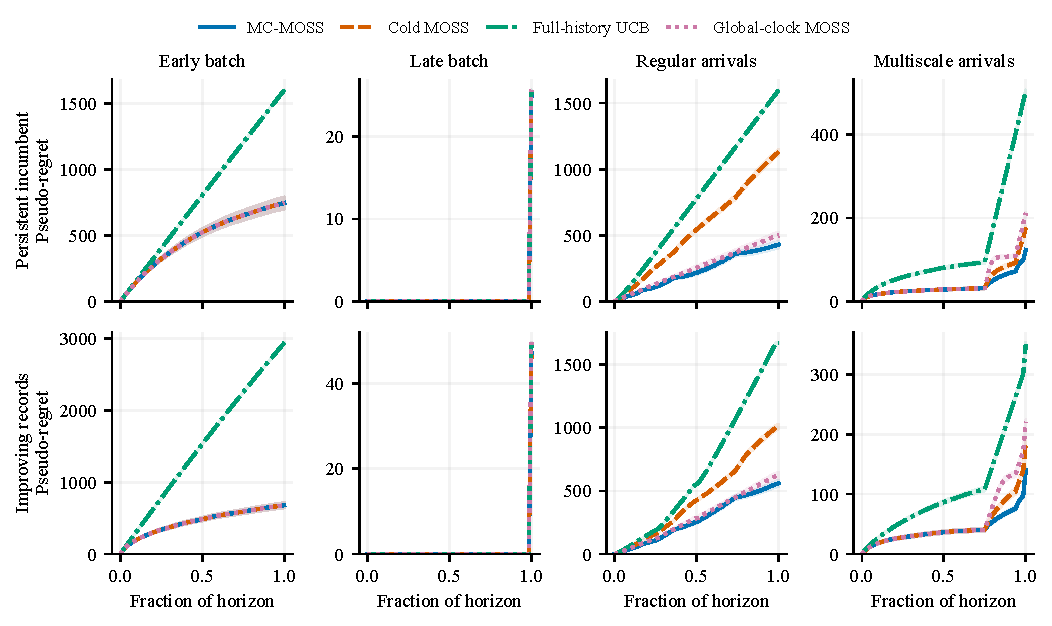
\includegraphics[width=\textwidth]{figures/fig_policy_comparison.pdf}
\caption{Mean cumulative pseudo-regret for the eight Bernoulli
environments. Shaded bands are the mean plus or minus 1.96 pointwise
Monte Carlo standard errors; they are not simultaneous confidence
bands. The first, second, and fourth methods coincide in the
early-batch panels. Vertical scales differ between panels.}
\label{fig:policy-comparison}
\end{figure}

Table~\ref{tab:regret} and Figure~\ref{fig:policy-comparison} show that history retention matters in the regular and multiscale schedules. For regular arrivals with a persistent incumbent, MC-MOSS has mean regret 429.4, compared with 1130.2 for Cold MOSS. The paired mean reduction is 700.8 with Monte Carlo standard error 14.9. MC-MOSS also has lower regret than the global/current comparison in these two schedules. That comparison changes both the clock and capacity calibration, so it does not isolate either effect. When every competitor arrives at time one, the three MOSS rules make identical decisions. The late-batch example gives a counterpoint: with a persistent incumbent, Cold MOSS has mean regret 24.83, versus 25.34 for MC-MOSS. The paired Cold-minus-MC difference is -0.51 with standard error 0.11. History retention therefore does not yield pointwise dominance, even in this small comparison.


These comparisons concern the specified environments and constants.
In particular, the fixed-gap environments need not be least favorable
for any schedule, and a small observed ratio of regret to
$\mathscr S_T$ does not estimate a minimax constant. The UCB comparison
also does not isolate history retention: UCB retains history but uses
a different exploration bonus.

\subsection{Restart costs and reproducibility checks}

We separately reproduce the deterministic restart example using
segment length $h=65{,}536$ and $m=1,\ldots,7$ segments. The first two
arms have rewards $1/2$ and $1/4$; segment $j=1,\ldots,m-1$ adds
$2^{j-1}$ arms with reward $1/2$. MC-MOSS pulls the unique inferior arm
94 times for every reported $m$, giving regret 23.5. Cold MOSS pulls it
94, 179, 255, 322, 380, 429, and 470 times, respectively; its regret
therefore reaches 117.5 at $m=7$. Figure~\ref{fig:structural-diagnostics}(a)
shows this finite repeated-exploration effect. These runs hold $h$
fixed; they do not numerically establish the asymptotic separation
proved using $h=2^{16m}$. The released analytic-bound table evaluates
the proved bounds for that latter family and labels those values as
bounds, not simulated trajectories.

\begin{figure}[t]
\centering
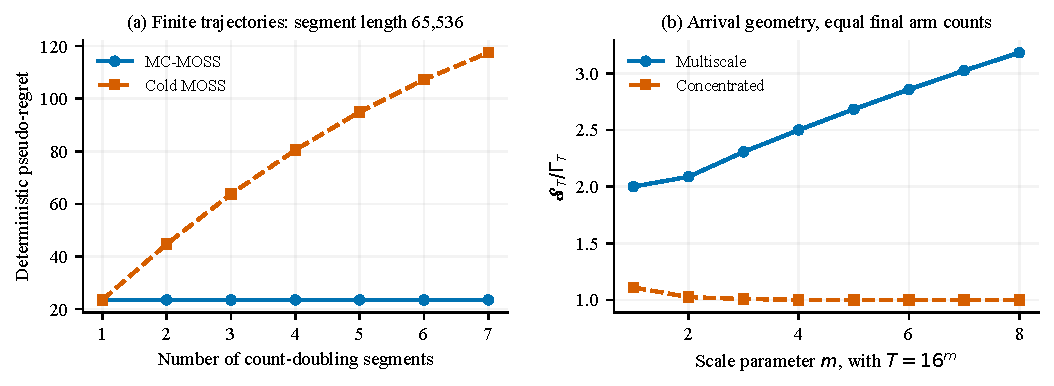
\includegraphics[width=\textwidth]{figures/fig_structural_diagnostics.pdf}
\caption{Two structural diagnostics. (a) Actual deterministic policy
trajectories with fixed segment length. (b) Exact geometric
calculations for the multiscale family with $T=16^m$ and a comparison
schedule with the same final arm count: $m+1$ competitors arrive at
time one and the rest arrive at time $T$. No policy simulation at
these exponential horizons is used in panel (b).}
\label{fig:structural-diagnostics}
\end{figure}

The computational audit also repeats 1,715 exhaustive small schedules
and 10,000 random schedules, checking capacity feasibility, primal--dual
agreement, spectral comparisons, clock charging, and the compatible
scale selection inequalities. An additional 2,001 online API steps
check the original interface and reward-range clipping example. Our
simulation implementation agrees with the original online MC-MOSS
interface on 6,168 individual actions. Forty-eight prefix checks hide
all labels arriving after the shorter endpoint and reproduce every
action on the common prefix for all four policies. The released
scripts, environment tables, seeds, raw replication results, paired
differences, and figure code permit regeneration of all numerical
claims above. These checks support reproducibility and implementation
consistency; the general statements rely on their analytic proofs.
